
% THIS IS AN EXAMPLE DOCUMENT FOR VLDB 2012
% based on ACM SIGPROC-SP.TEX VERSION 2.7
% Modified by  Gerald Weber <gerald@cs.auckland.ac.nz>
% Removed the requirement to include *bbl file in here. (AhmetSacan, Sep2012)
% Fixed the equation on page 3 to prevent line overflow. (AhmetSacan, Sep2012)

\documentclass{vldb}
\usepackage{graphicx}
\usepackage{balance}  % for  \balance command ON LAST PAGE  (only there!)

% ****************** sungsoo's packages ****************************************
\usepackage{times}
%                              My Commands
\newcommand{\bi}{\begin{itemize}}
\newcommand{\ei}{\end{itemize}}
\newcommand{\be}{\begin{enumerate}}
\newcommand{\ee}{\end{enumerate}}
\newcommand{\ii}{\item}
\newtheorem{Def}{Definition}
\newtheorem{Lem}{Lemma}
\usepackage{algorithm}
\usepackage{algorithmicx}
\usepackage{algpseudocode}

%\usepackage[]{algorithm2e}

\usepackage{graphicx}
\graphicspath{%
        {converted_graphics/}
        {./images/}
}
\usepackage{hyperref}
\usepackage{listings}
\usepackage{longtable}

% ****************** the following is needed for syntax highlighting
\usepackage{color}

\definecolor{dkgreen}{rgb}{0,0.6,0}
\definecolor{gray}{rgb}{0.5,0.5,0.5}
\definecolor{mauve}{rgb}{0.58,0,0.82}

\lstset{ %
  language=Java,                  % the language of the code
  basicstyle=\scriptsize,       % the size of the fonts that are used for the code
  numbers=left,                   % where to put the line-numbers
  numberstyle=\tiny\color{gray},  % the style that is used for the line-numbers
  stepnumber=1,                   % the step between two line-numbers. If it's 1, each line 
                                  % will be numbered
  numbersep=3.8pt,                  % how far the line-numbers are from the code
  backgroundcolor=\color{white},  % choose the background color. You must add \usepackage{color}
  showspaces=false,               % show spaces adding particular underscores
  showstringspaces=false,         % underline spaces within strings
  showtabs=false,                 % show tabs within strings adding particular underscores
  frame=false,                   % adds a frame around the code
  rulecolor=\color{black},        % if not set, the frame-color may be changed on line-breaks within not-black text (e.g. commens (green here))
  tabsize=2,                      % sets default tabsize to 2 spaces
  captionpos=b,                   % sets the caption-position to bottom
  breaklines=true,                % sets automatic line breaking
  breakatwhitespace=false,        % sets if automatic breaks should only happen at whitespace
  title=\lstname,                 % show the filename of files included with \lstinputlisting;
                                  % also try caption instead of title
  keywordstyle=\color{blue},          % keyword style
  commentstyle=\color{dkgreen},       % comment style
  stringstyle=\color{mauve},         % string literal style
  escapeinside={\%*}{*)},            % if you want to add a comment within your code
  morekeywords={*,...}               % if you want to add more keywords to the set
}
% ****************** end of sungsoo's packages ****************************************


\begin{document}

% ****************** TITLE ****************************************

%\title{A Sample {\ttlit Proceedings of the VLDB Endowment} Paper in LaTeX
%Format\titlenote{for use with vldb.cls}}

\title{Apache Hive on Apache Spark: Motivations and Design Principles}

% possible, but not really needed or used for PVLDB:
%\subtitle{[Extended Abstract]
%\titlenote{A full version of this paper is available as\textit{Author's Guide to Preparing ACM SIG Proceedings Using \LaTeX$2_\epsilon$\ and BibTeX} at \texttt{www.acm.org/eaddress.htm}}}

% ****************** AUTHORS **************************************

% You need the command \numberofauthors to handle the 'placement
% and alignment' of the authors beneath the title.
%
% For aesthetic reasons, we recommend 'three authors at a time'
% i.e. three 'name/affiliation blocks' be placed beneath the title.
%
% NOTE: You are NOT restricted in how many 'rows' of
% "name/affiliations" may appear. We just ask that you restrict
% the number of 'columns' to three.
%
% Because of the available 'opening page real-estate'
% we ask you to refrain from putting more than six authors
% (two rows with three columns) beneath the article title.
% More than six makes the first-page appear very cluttered indeed.
%
% Use the \alignauthor commands to handle the names
% and affiliations for an 'aesthetic maximum' of six authors.
% Add names, affiliations, addresses for
% the seventh etc. author(s) as the argument for the
% \additionalauthors command.
% These 'additional authors' will be output/set for you
% without further effort on your part as the last section in
% the body of your article BEFORE References or any Appendices.

\numberofauthors{1} %  in this sample file, there are a *total*
% of EIGHT authors. SIX appear on the 'first-page' (for formatting
% reasons) and the remaining two appear in the \additionalauthors section.

\author{
% You can go ahead and credit any number of authors here,
% e.g. one 'row of three' or two rows (consisting of one row of three
% and a second row of one, two or three).
%
% The command \alignauthor (no curly braces needed) should
% precede each author name, affiliation/snail-mail address and
% e-mail address. Additionally, tag each line of
% affiliation/address with \affaddr, and tag the
% e-mail address with \email.
%
% 1st. author
\alignauthor
Sung-Soo Kim\\ %\titlenote{Dr.~Trovato insisted his name be first.}\\
       \affaddr{Data Management Research Section}\\
       \affaddr{Electronics and Telecommunications Research Institute}\\
       \affaddr{128 Gajeong-ro, Yuseong-gu}\\
       \affaddr{Daejeon, South Korea}\\
       \email{\normalsize \it sungsoo@etri.re.kr}
% 2nd. author
%\alignauthor
%G.K.M. Tobin\titlenote{The secretary disavows
%any knowledge of this author's actions.}\\
%       \affaddr{Institute for Clarity in Documentation}\\
%       \affaddr{P.O. Box 1212}\\
%       \affaddr{Dublin, Ohio 43017-6221}\\
%       \email{webmaster@marysville-ohio.com}
% 3rd. author
%\alignauthor Lars Th{\Large{\sf{\o}}}rv{$\ddot{\mbox{a}}$}ld\titlenote{This author is the
%one who did all the really hard work.}\\
%       \affaddr{The Th{\large{\sf{\o}}}rv{$\ddot{\mbox{a}}$}ld Group}\\
%       \affaddr{1 Th{\large{\sf{\o}}}rv{$\ddot{\mbox{a}}$}ld Circle}\\
%       \affaddr{Hekla, Iceland}\\
%       \email{larst@affiliation.org}
%\and  % use '\and' if you need 'another row' of author names
% 4th. author
%\alignauthor Lawrence P. Leipuner\\
%       \affaddr{Brookhaven Laboratories}\\
%       \affaddr{Brookhaven National Lab}\\
%       \affaddr{P.O. Box 5000}\\
%       \email{lleipuner@researchlabs.org}
% 5th. author
%\alignauthor Sean Fogarty\\
%       \affaddr{NASA Ames Research Center}\\
%       \affaddr{Moffett Field}\\
%       \affaddr{California 94035}\\
%       \email{fogartys@amesres.org}
% 6th. author
%\alignauthor Charles Palmer\\
%       \affaddr{Palmer Research Laboratories}\\
%       \affaddr{8600 Datapoint Drive}\\
%       \affaddr{San Antonio, Texas 78229}\\
%       \email{cpalmer@prl.com}
}
% There's nothing stopping you putting the seventh, eighth, etc.
% author on the opening page (as the 'third row') but we ask,
% for aesthetic reasons that you place these 'additional authors'
% in the \additional authors block, viz.
%\additionalauthors{Additional authors: John Smith (The Th{\o}rv\"{a}ld Group, {\texttt{jsmith@affiliation.org}}), Julius P.~Kumquat
%(The \raggedright{Kumquat} Consortium, {\small \texttt{jpkumquat@consortium.net}}), and Ahmet Sacan (Drexel University, {\small \texttt{ahmetdevel@gmail.com}})}
%\date{30 July 1999}
% Just remember to make sure that the TOTAL number of authors
% is the number that will appear on the first page PLUS the
% number that will appear in the \additionalauthors section.


\maketitle

\begin{abstract}
Two of the most vibrant communities in the Apache Hadoop
ecosystem are now working together to bring users a Hive-on-Spark option
that combines the best elements of both.
% There are many different roles on a data warehouse project that are filled by systems professionals. Many roles are consistent regardless of what kind of system is being developed. In this technical report, we describe the IT roles and responsibilities (R\&R) for a data warehouse project.
\end{abstract}

\section{Introduction}

%\begin{figure}[htb]
%\centering
%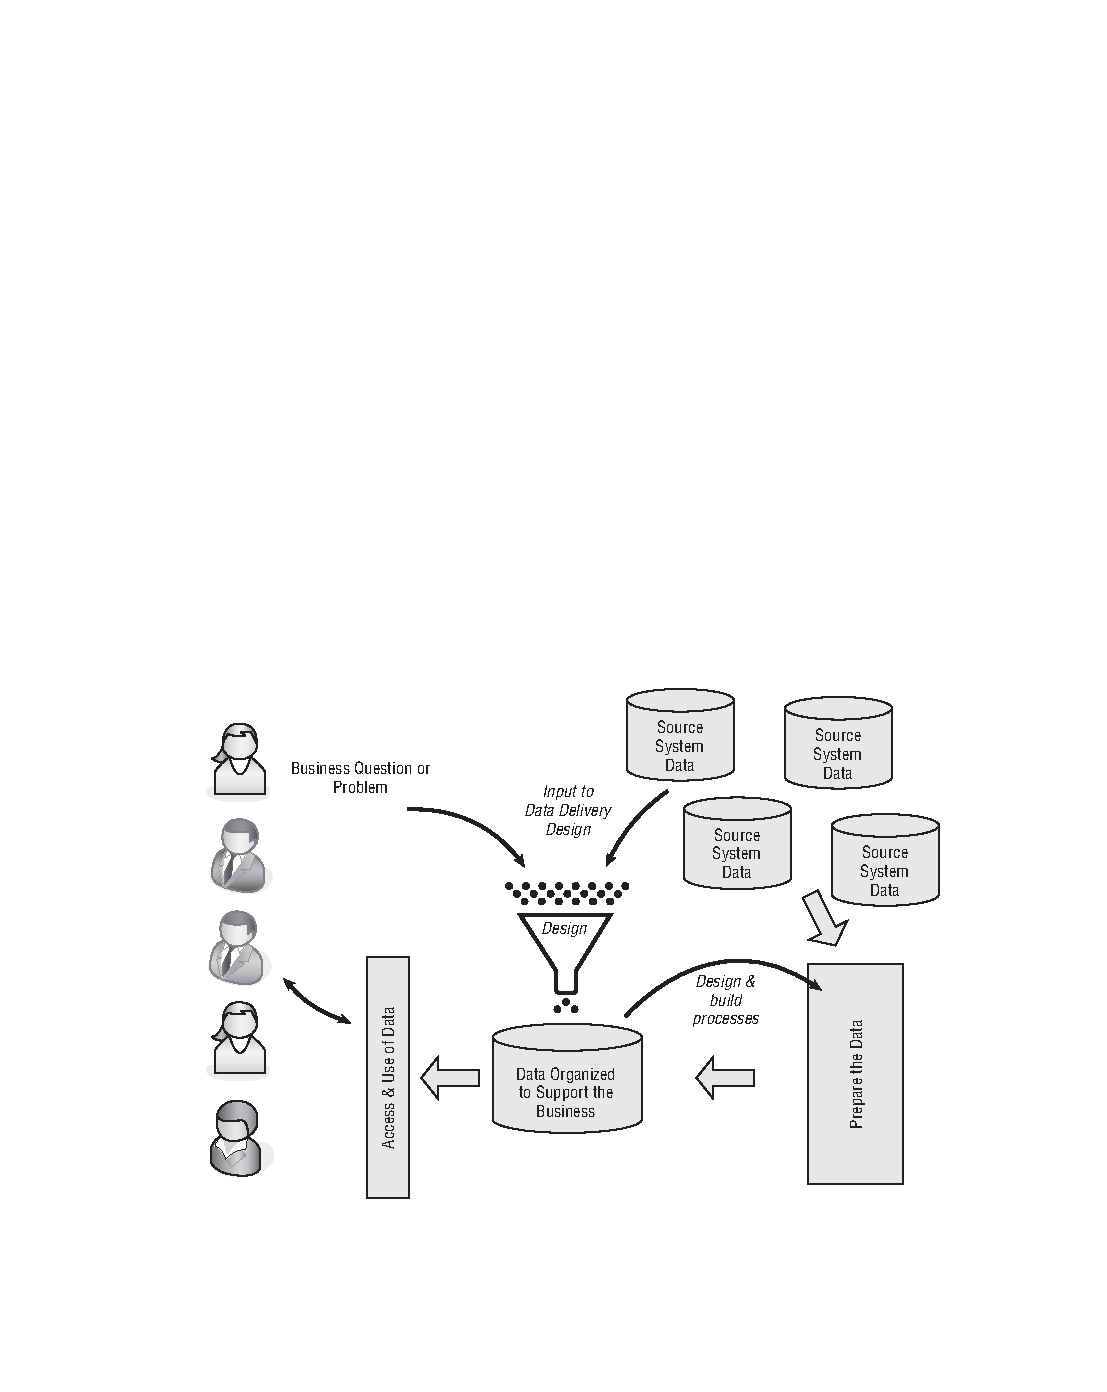
\includegraphics[width=0.48\textwidth]{datawarehouse}
%\caption{Optimal data warehouse design and development sequence}
%\label{fig:datawarehouse}
%\end{figure}

Apache Hive is a popular SQL interface for batch processing and ETL
using Apache Hadoop. Until recently, MapReduce was the only execution
engine in the Hadoop ecosystem, and Hive queries could only run on
MapReduce. But today, alternative execution engines to MapReduce are
available --- such as \href{http://spark.apache.org}{Apache Spark} and
\href{http://incubator.apache.org/projects/tez.html}{Apache Tez
(incubating)}.

Although Spark is relatively new to the Hadoop ecosystem, its
\href{https://cwiki.apache.org/confluence/display/SPARK/Powered+By+Spark}{adoption
has been meteoric}. An open-source data analytics cluster computing
framework, Spark is built outside of Hadoop's two-stage MapReduce
paradigm but runs on top of HDFS. Because of its successful approach,
Spark has quickly gained momentum and become established as an
attractive choice for the future of data processing in Hadoop.

In this post, you'll get an overview of the motivations and technical
details behind some very exciting news for Spark and Hive users: the
fact that the Hive and Spark communities are joining forces to
collaboratively introduce Spark as a new execution engine option for
Hive, alongside MapReduce and Tez (see
\href{https://issues.apache.org/jira/browse/HIVE-7292}{HIVE-7292}).

\section{Motivation and Approach}

Here are the two main motivations for enabling Hive to run on Spark:

\begin{itemize}
\itemsep1pt\parskip0pt\parsep0pt
\item
  \textbf{To improve the Hive user experience}\\ Hive queries will run
  faster, thereby improving user experience. Furthermore, users will
  have access to a robust, non-MR execution engine that has already
  proven itself to be a leading option for data processing as well as
  streaming, and which is among the
  \href{https://www.ohloh.net/orgs/apache}{most active projects} across
  all of Apache from contributor and commit standpoints.
\item
  \textbf{To streamline operational management for Spark shops}\\
  Hive-on-Spark will be very valuable for users who are already using
  Spark for other data-processing and machine-learning needs.
  Standardizing on one execution back end is also convenient for
  operational management, making it easier to debug issues and create
  enhancements.
\end{itemize}

Superficially, this project's goals look similar to those of Shark or
Spark SQL, which are separate projects that reuse the Hive front end to
run queries using Spark. However, this design adds Spark into Hive,
parallel to MapReduce and Tez, as another backend execution
engine.~Thus, existing Hive jobs continue to run as-is transparently on
Spark.

The key advantage of this approach is to leverage all the existing
integration on top of Hive, including ODBC/JDBC, auditing,
authorization, and monitoring. Another advantage is that it will have no
impact on Hive's existing code path and thus no functional or
performance effects. Users choosing to run Hive on either MapReduce or
Tez will have the same functionality and code paths they have today ---
thus, the Hive user community will be in the great position of being
able to choose among MapReduce, Tez, or Spark as a back end. In
addition, maintenance costs will be minimized so the Hive community
needn't make specialized investments for Spark.

Meanwhile, users opting for Spark as the execution engine will
automatically have all the rich functional features that Hive provides.
Future features (such as new data types, UDFs, logical optimization, and
so on ) added to Hive should become automatically available to those
users, without any customization work to be done in Hive's Spark
execution engine.

\section{Overall Functionality}

To use Spark as an execution engine in Hive, you would set the
following:

\texttt{set hive.execution.engine=spark;}

The default value for this configuration is still ``\texttt{mr}''. Hive
will continue to work on MapReduce as-is on clusters that don't have
Spark on them. When Spark is configured as Hive's execution, a few
configuration variables will be introduced, such as the master URL of
the Spark cluster.

The new execution engine should support all Hive queries without any
modification. Query results should be functionally equivalent to those
from either MapReduce or Tez. In addition, existing functionality
related to the execution engine should also be available, including the
following:

\begin{itemize}
\itemsep1pt\parskip0pt\parsep0pt
\item
  Hive will display a task execution plan that's similar to that being
  displayed by the \texttt{explain} command for MapReduce and Tez. ~~~~
\item
  Hive will give appropriate feedback to the user about progress and
  completion status of the query when running queries on Spark.
\item
  The user will be able to get statistics and diagnostic information as
  before (counters, logs, and debug info on the console).
\end{itemize}

\section{Hive-Level Design}

As noted previously, this project takes a different approach from that
of Shark in that SQL semantics will be not implemented using Spark's
primitives, but rather MapReduce ones that will be executed in Spark.

The main work to implement the Spark execution engine for Hive has two
components: query planning, where Hive operator plan from semantic
analyzer is further translated a task plan that Spark can execute; and
query execution, where the generated Spark plan is executed in the Spark
cluster. There are other miscellaneous yet indispensable functional
pieces involving monitoring, counters, statistics, and so on, but for
brevity, we will only address the main design considerations here.

\hyperdef{}{}{\subparagraph{Query Planning}}

Currently, for a given user query, Hive's semantic analyzer generates an
operator plan that comprises a graph of logical operators such as
\texttt{TableScanOperator}, \texttt{ReduceSink}, \texttt{FileSink},
\texttt{GroupByOperator}, and so on. \texttt{MapReduceCompiler} compiles
a graph of \texttt{MapReduceTask}s and other helper tasks (such as
\texttt{MoveTask}) from the logical operator plan. Tez behaves
similarly, yet generates a \texttt{TezTask} that combines otherwise
multiple MapReduce tasks into a single Tez task.

For Spark, we will introduce \texttt{SparkCompiler} parallel to
\texttt{MapReduceCompiler} and \texttt{TezCompiler}. Its main
responsibility is to compile from the Hive logical operator plan a plan
that can be executed on Spark. Thus, we will have \texttt{SparkTask},
depicting a job that will be executed in a Spark cluster, and
\texttt{SparkWork}, describing the plan of a Spark task. Thus,
\texttt{SparkCompiler} translates a Hive's operator plan into a
\texttt{SparkWork} instance. During the task plan generation,
\texttt{SparkCompiler} may also perform physical optimizations suitable
for Spark.~~~

\hyperdef{}{}{\subparagraph{Job Execution}}

A \texttt{SparkTask} instance can be executed by Hive's task execution
framework in the same way as for other tasks. Internally, the
\texttt{SparkTask.execute()} method will make RDDs and functions out of
a \texttt{SparkWork} instance, and submit the execution to the Spark
cluster via a Spark client.

Once the Spark work is submitted to the Spark cluster, the Spark client
will continue to monitor the job execution and report progress. A Spark
job can be monitored via \texttt{SparkListener} APIs.

With \texttt{SparkListener} APIs, we will add a \texttt{SparkJobMonitor}
class that handles printing of status as well as reporting the final
result. This class provides similar functions as
\texttt{HadoopJobExecHelper} used for MapReduce processing, or
\texttt{TezJobMonitor} used for Tez job processing, and will also
retrieve and print the top-level exception thrown at execution time in
case of job failure.

Spark job submission is done via a \texttt{SparkContext} object that's
instantiated with the user's configuration. When a \texttt{SparkTask} is
executed by Hive, such a context object is created in the current user
session. With the context object, RDDs corresponding to Hive tables are
created and \texttt{MapFunction} and \texttt{ReduceFunction} (more
details below) are built from Hive's \texttt{SparkWork} and applied to
the RDDs. Job execution is triggered by applying a \texttt{foreach()}
transformation on the RDDs with a dummy function.

\section{Main Design Considerations}}

Hive's operator plan is based on MapReduce paradigm, and traditionally,
a query's execution contains a list of MapReduce jobs. Each MapReduce
job consists of map-side processing starting from Hive's
\texttt{ExecMapper} and reduce-side processing starting from
\texttt{ExecReducer}, and MapReduce provides inherent shuffling,
sorting, and grouping between the map-side and the reduce-side. The
input to the whole processing pipeline are the folders and files
corresponding to the table.

Because we will reuse Hive's operator plan but perform the same data
processing in Spark, the execution plan will be built in Spark
constructs such as RDD, function, and transformation. This approach is
outlined below.

\hyperdef{}{}{\subparagraph{Table as RDD}}

A Hive table is simply a bunch of files and folders on HDFS. Spark
primitives are applied to RDDs. Thus, naturally, Hive tables will be
treated as RDDs in the Spark execution engine.

\hyperdef{}{}{\subparagraph{MapFunction}}

The above mentioned \texttt{MapFunction} will be made from
\texttt{MapWork}; specifically, the operator chain starting from
\texttt{ExecMapper.map()} method. \texttt{ExecMapper} class implements
MapReduce Mapper interface, but the implementation in Hive contains some
code that can be reused for Spark. Therefore, we will extract the common
code into a separate class, \texttt{MapperDriver}, to be shared by
MapReduce as well as Spark.

\hyperdef{}{}{\subparagraph{ReduceFunction}}

Similarly, \texttt{ReduceFunction} will be made of \texttt{ReduceWork}
instance from \texttt{SparkWork}. To Spark, \texttt{ReduceFunction} is
no different than \texttt{MapFunction}, but the function's
implementation will be different, and made of the operator chain
starting from \texttt{ExecReducer.reduce()}. Also, because some code in
\texttt{ExecReducer} will be reused, we will extract the common code
into a separate class, \texttt{ReducerDriver}, for sharing by both
MapReduce and Spark.

\hyperdef{}{}{\subparagraph{Shuffle, Group, and Sort}}

While this functionality comes for ``free'' along with MapReduce, we
will need to provide an equivalent for Spark. Fortunately, Spark
provides a few transformations that are suitable for replacing
MapReduce's shuffle capability, such as \texttt{partitionBy},
\texttt{groupByKey}, and \texttt{sortByKey}. Transformation
\texttt{partitionBy} does pure shuffling (no grouping or sorting),
\texttt{groupByKey} does shuffling and grouping, and
\texttt{sortByKey()} does shuffling plus sorting. Therefore, for each
\texttt{ReduceSinkOperator} in \texttt{SparkWork}, we will need to
inject one of the transformations.

Having the capability to selectively choose the exact shuffling behavior
provides opportunities for optimization. For instance, Hive's
\texttt{groupBy} doesn't require the key to be sorted, but MapReduce
does. In contrast, in Spark, one can choose \texttt{sortByKey} only if
key order is important (such as for SQL \texttt{ORDER BY}).

\hyperdef{}{}{\subparagraph{Multiple Reduce Stages}}

Whenever a query has multiple \texttt{ReduceSinkOperator} instances,
Hive will break the plan apart and submit one MR job per sink. All the
MR jobs in this chain need to be scheduled one-by-one, and each job has
to re-read the output of the previous job from HDFS and shuffle it. In
Spark, this step is unnecessary: multiple map functions and reduce
functions can be concatenated. For each \texttt{ReduceSinkOperator}, a
proper shuffle transformation needs to be injected as explained above.

\section{Conclusion}}

Based on the above, you will likely recognize that although Hive on
Spark is simple and clean in terms of functionality and design, the
implementation will take some time. Therefore, the community will take a
phased approach, with all basic functionality delivered in a Phase 1 and
optimization and improvements ongoing over a longer period of time.
(Precise number of phases and what each will entail are under
discussion.)

Most important, the Hive and Spark communities will work together
closely to achieve this technical vision and resolve any obstacles that
might arise --- with the end result being the availability to Hive users
of an execution engine that improves performance as well as unifies
batch and stream processing.

\bibliographystyle{abbrv}
\bibliography{sqlonhadoop}

\end{document}
